\documentclass{article}\usepackage[]{graphicx}\usepackage[]{color}
%% maxwidth is the original width if it is less than linewidth
%% otherwise use linewidth (to make sure the graphics do not exceed the margin)
\makeatletter
\def\maxwidth{ %
  \ifdim\Gin@nat@width>\linewidth
    \linewidth
  \else
    \Gin@nat@width
  \fi
}
\makeatother

\definecolor{fgcolor}{rgb}{0.345, 0.345, 0.345}
\newcommand{\hlnum}[1]{\textcolor[rgb]{0.686,0.059,0.569}{#1}}%
\newcommand{\hlstr}[1]{\textcolor[rgb]{0.192,0.494,0.8}{#1}}%
\newcommand{\hlcom}[1]{\textcolor[rgb]{0.678,0.584,0.686}{\textit{#1}}}%
\newcommand{\hlopt}[1]{\textcolor[rgb]{0,0,0}{#1}}%
\newcommand{\hlstd}[1]{\textcolor[rgb]{0.345,0.345,0.345}{#1}}%
\newcommand{\hlkwa}[1]{\textcolor[rgb]{0.161,0.373,0.58}{\textbf{#1}}}%
\newcommand{\hlkwb}[1]{\textcolor[rgb]{0.69,0.353,0.396}{#1}}%
\newcommand{\hlkwc}[1]{\textcolor[rgb]{0.333,0.667,0.333}{#1}}%
\newcommand{\hlkwd}[1]{\textcolor[rgb]{0.737,0.353,0.396}{\textbf{#1}}}%
\let\hlipl\hlkwb

\usepackage{framed}
\makeatletter
\newenvironment{kframe}{%
 \def\at@end@of@kframe{}%
 \ifinner\ifhmode%
  \def\at@end@of@kframe{\end{minipage}}%
  \begin{minipage}{\columnwidth}%
 \fi\fi%
 \def\FrameCommand##1{\hskip\@totalleftmargin \hskip-\fboxsep
 \colorbox{shadecolor}{##1}\hskip-\fboxsep
     % There is no \\@totalrightmargin, so:
     \hskip-\linewidth \hskip-\@totalleftmargin \hskip\columnwidth}%
 \MakeFramed {\advance\hsize-\width
   \@totalleftmargin\z@ \linewidth\hsize
   \@setminipage}}%
 {\par\unskip\endMakeFramed%
 \at@end@of@kframe}
\makeatother

\definecolor{shadecolor}{rgb}{.97, .97, .97}
\definecolor{messagecolor}{rgb}{0, 0, 0}
\definecolor{warningcolor}{rgb}{1, 0, 1}
\definecolor{errorcolor}{rgb}{1, 0, 0}
\newenvironment{knitrout}{}{} % an empty environment to be redefined in TeX

\usepackage{alltt}

  % Packages
  %% Setting nice page margins
  \usepackage{geometry}
    \geometry{margin=20mm}
  %% Hyperlink (cross/page) references
  \usepackage{hyperref}
  %% Colour
  \usepackage[dvipsnames]{xcolor}
      \definecolor{col1}{HTML}{873B70}
        \definecolor{col1light}{HTML}{d8a6c9}
      \definecolor{col2}{HTML}{7086BF}
        \definecolor{col2dark}{HTML}{374a7b}
  %% Notes below charts
  \usepackage[capposition=top]{floatrow}
      \newcommand{\wnote}[1]{\vspace{-5mm} \floatfoot{\centering{\textit{Note: #1}}}}
  %% Maths
  \usepackage{amsmath}
  %% Add code to LaTeX document
  \usepackage{listings}
  
  %% Fix footnote-drift problem
  \usepackage[bottom]{footmisc}

  %% For title creation
  \usepackage{blindtext}

 % Changing some defaults for ease-of-readability
 \setlength{\parindent}{0pt} %% no indent
 \setlength{\parskip}{5mm}  %% paragraph spacing
    
% Define some common phrases for consistency
  \newcommand{\ie}{\textit{i.e.}}
  \newcommand{\eg}{\textit{e.g.}}



\title{Time Series Analysis and Forecasting (ECOM30004): Assignment 1}
\date{2018\\ August}
\author{Will Mackey\\ 790114}
\IfFileExists{upquote.sty}{\usepackage{upquote}}{}
\begin{document}
\maketitle


%% R installation



\section{Conceptual question}

\subsection{} %%Question 1.1
    The first structural-break model is:
        \begin{align*}
          y_t  &= \alpha_0 + \alpha_1 DI_{t} + U_{1t}    \tag*{where $U_{1t}$ is noise; \textit{(i)}} \\
          DI_t &=                                      \tag*{where $1< T_B <T$}
          \begin{cases}
            0 \text{\quad  if \quad} t \leq T_B \\
            1 \text{\quad  if \quad} t >    T_B
          \end{cases}
        \end{align*}
    When the structural break occurs for model ($i$), the change in expected output is the post-break expectation $E[y_{t,DI_{t}=1}]$ less the pre-break expectation $E[y_{t,DI_{t}=0}]$, shown below.

    From:
        \begin{align*}
          E[y_{t,DI_{t}=0}] &= E[\alpha_0] + E[U_{1t}]    \tag*{where $E[U_{1t}]=0$} \\ 
                      &= \alpha_0                         \tag*{as $\alpha_0$ is a constant}
        \end{align*}
    to:
        \begin{align*}
          E[y_{t,DI_{t}=1}] &= E[\alpha_0 + \alpha_1 + U_{1t}]                                 \\ 
                            &= E[\alpha_0] + E[\alpha_1]   + E[U_{1t}]    \tag*{where $E[U_{1t}]=0$} \\ 
                            &= \alpha_0  + \alpha_1
        \end{align*}
    giving:
        \begin{align*}
          E[y_{t,DI_{t}=1}] - E[y_{t,DI_{t}=0}] &= \alpha_1
        \end{align*}
    Or, the difference in expected $y_t$ is $\alpha_1$. This shows that model ($i$), which is simulated in Figure \ref{chart11} alongside model ($ii$), could represent a time-invariant variable that changes \textit{levels} due to a shock. For example, productivity growth ($y_t$) of an established industry that experiences a permanent negative shock ($a_1<0$) when a competitor enters the market at time $T_B$.

    \vspace{5mm}

    The second structual-break model is:
        \begin{align*} 
        y_t  &= \beta_{0} + \beta_{1} t + \beta_{2} DI_{t} + U_{2t}    \tag*{where $U_{2t}$ is noise, \textit{(ii)}} \\ 
        DI_t &=                                      \tag*{where $1< T_B <T$}
        \begin{cases}
          0 \text{\quad  if \quad}         t \leq T_B \\
          t - T_{B} \text{\quad  if \quad} t >    T_B
        \end{cases}
      \end{align*}

    Similarly, when the structual break occurs, the expected output changes by the post-break expectation $E[y_{t,DT_{t}=t-T_B}]$ less the pre-break expectation $E[y_{t,DT_{t}=0}]$.

    From:
        \begin{align*}
          E[y_{t,DT_{t}=0}] &= E[\beta_0 +   \beta_1 t + U_{2t}]    \tag*{where $E[U_{2t}]=0$} \\ 
                            &= \beta_0 + \beta_1 t
        \end{align*}

    to:
        \begin{align*}
          E[y_{t,DT_{t}=0}] &= E[\beta_0 + \beta_1 t + \beta_2 (t - T_{B}) + U_{2t}]    \tag*{where $E[U_{2t}]=0$} \\ 
                            &= \beta_0 + \beta_1 t + \beta_2 (t - T_{B}) \\ 
        \end{align*}

    giving the change:
        \begin{align*}
          E[y_{t,DT_{t}=(t-T_{B})}] - E(y_{t,DI_{t}=0}) &= \beta_2 (t - T_{B})
        \end{align*}
    Or, the difference in expected $y_t$ is the estimated time-dependant linear trend with coefficent $\beta_2$. Unlike model ($i$), model ($ii$) is time-variant with a time-dependant structural break: the pre-break trend is dependant on time, and this `relationship' with time changes significantly after the break. It could represent high- and increasing-growth ($\beta_{1}>0$) in university student numbers at Australian institutions after a the introduction of the demand-driven system at time $T_B$. This is, very roughly, shown in Figure \ref{chart11}.\footnote{One would have to assume monthly data-collection on enrolments and a lack of a semester-based enrolment system for this figure to match the example well. Strong imagination required.}





    \begin{figure}
    \caption{Models ($i$) and ($ii$)}
        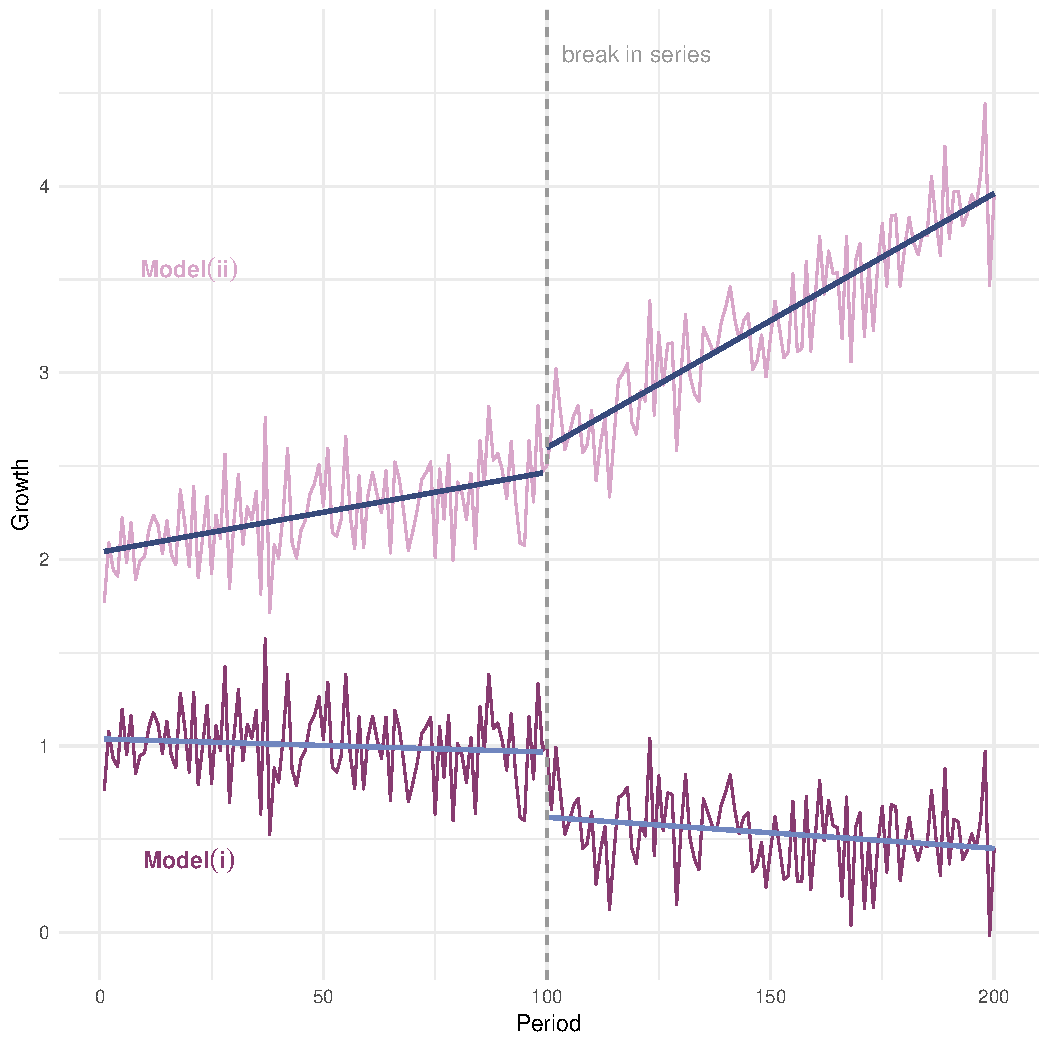
\includegraphics[width=.8\columnwidth]{atlas/chart11.pdf}
        \label{chart11} 
      \wnote{The two models simulated with the same normally distributed errors over 200 time periods. The structural break occurs at t=100. Parameters for model (i): $\alpha_0 = 1$ and $\alpha_1 = -0.5$; for model (ii): $\beta_0 = 2$, $\beta_1 = 0.005$ and $\beta_2 = 0.01$. Linear trends with breaks are shown for \textcolor{col2}{model (i)} and \textcolor{col2dark}{model (ii)}.}
    \end{figure}


\newpage

\subsection{} %%Question 1.2

    Model A is time-variant with one structural break and can be expressed as
      \begin{align*}
        p_{t} = \alpha_0 + \alpha_1 t + \alpha_2 T_{B,1} + U_{1t}
      \end{align*}
    Model B \textit{likely} has six structural breaks, denoted in the following general-form model as $T_{B,1}$ through $T_{B,6}$.\footnote{Although it may have seven if there is one at M12; but we'll assume six for the remainder of the question.}
      \begin{align*}
        p_{t} = \beta_0 + \beta_1 t &+ \beta_2 T_{B,1}  \\
                                    &+ \beta_3 T_{B,2} \\
                                    &+ \beta_4 T_{B,3} \\
                                    &+ \beta_5 T_{B,4} \\
                                    &+ \beta_6 T_{B,5} \\
                                    &+ \beta_7 T_{B,6} \\
                                    &+ U_{2t}
      \end{align*}
    Model B increases the information in (number of variables of) the model, and \textit{necessarily} increases its ``fit'' ($R^2$).\footnote{See \textit{Econometrics 1} for a detailed discussion.} But this is at the cost of degrees of freedom, and will produce an overfitted model. The coefficients of $T_{B,n}$ would the noise of the data rather than any proper relationship with population events. As the number of breaks approaches the number of observations $n \xrightarrow\ N$ we lose the ability to model structural change; it would be like introducing a dummy variable for each period of observation (day, in this case), which would provide a perfect summary of the Yahoo share-price in the past but provide no information of any other trend. The model would fail to be deterministic --- have a clear relationship with time $t$ --- as it is crowded-out by the every-day-break variables.


  \newpage  
\section{Empirical question}

\subsection{}\label{subsec21}




    
        \begin{figure}[h!]
        \caption{Daily log-volume of shares traded on the S\&P/ASX 200}
            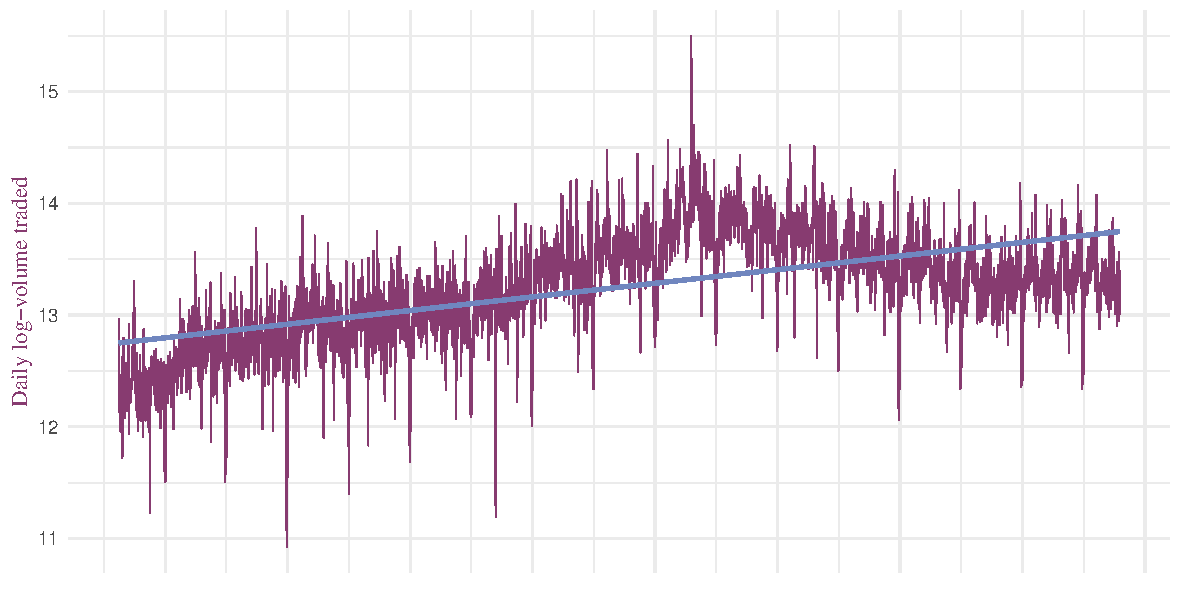
\includegraphics[width=.8\columnwidth]{atlas/chart21.pdf}
            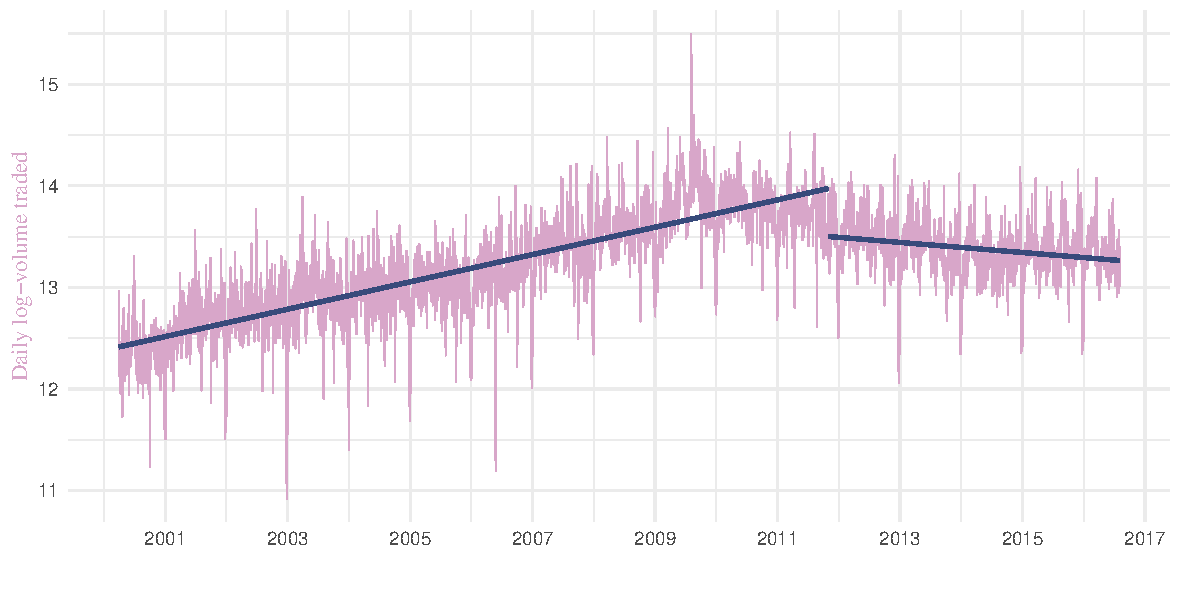
\includegraphics[width=.8\columnwidth]{atlas/chart21_break.pdf}
            \label{chart21} 
          \wnote{The linear trend without a break is shown in the first panel in \textcolor{col2}{blue}. The daily log-volume is repeated in the second panel, with a pre- and post-Chi-X trend in \textcolor{col2dark}{dark blue}}
        \end{figure}

The variable volume \(volume_{t}\) is units of thousands of shares traded daily. The log of volume \(log(volume_{t})\) is plotted against time in Figure \ref{chart21}. The time-series show a deterministic trend of log-volume traded. there is are clear relationships with time. There is strong growth in trading volume between mid-2000 and late-2009. From 2010 there is a `tempering' for 18 months followed by a decrease in trading between mid-2011 and late-2016, the end of the series.\footnote{This decrease is notable given the population increase in Australia --- a positive contributing factor of trading-volume --- over this period. It might be interesting to look at, say, the trend in trading-volume per person.} From the plot, there is a clear relationship between time and log-volume traded.

\newpage
\subsection{}\label{subsec22}
A model for log volume is shown in (1) below.
    \begin{align*} \label{eq22} 
    \log{vol_t}  = \beta_{0} + \beta_{1} t + \beta_{2} DT_{t} &+ \beta_{3,1} Mon_{t} \tag*{(1)} \\ 
                                                              &+ \beta_{3,2} Tue_{t} \\
                                                              &+ \beta_{3,3} Wed_{t} \\
                                                              &+ \beta_{3,4} Thu_{t} \\
                                                              &+ \beta_{3,5} Fri_{t} \\
                                                      &+ U_{t}
    \end{align*}
  Model (1) allows for three broad effects: the overall deterministic structure is modelled through $t$; $DT_{t}$ allows for a potential structural break, visually shown in the second panel of Part \ref{subsec21}, after the introduction of the Chi-X trading platform; and day-of-the-week effects are modelled through the dummy variables $Mon$-$Fri$, where $Mon$ takes a value of $1$ if the day is is Monday, $Tue$ for Tuesday, and so on.\footnote{Monday is the day-of-the-week chosen to be excluded due to autocorrelation. Note also that seasonal effects would add to the model, but are excluded for simplicity.} $U_{t}$ is white noise.





\newpage
\subsection{} \label{subsec23} %% Question 2.3

  Model \label{eq22} was estimated in \texttt{R}, and its results are presented in Table 1.\footnote{Full, reproducable code for this assignment can be found at  \url{www.github.com/wfmackey/timeseries-coursework/tree/master/assignment1} (only made public after the due date).}




%% Table of regression results
\begin{table}[h!] \centering 
      \caption{Results of Model (1)} 
      \label{tab1} 
      \begin{tabular}{@{\extracolsep{5pt}}lc} 
          \\[-1.8ex]\hline 
          \hline \\[-1.8ex] 
           & \multicolumn{1}{c}{\textit{Dependent variable:}} \\ 
          \\[-1.8ex] & \multicolumn{1}{c}{$ln(vol)$} \\ 
          \\[-1.8ex] & (1) \\ 
          \hline \\[-1.8ex] 
           t & 0.00046$^{***}$ \\ 
            & (0.00001) \\ 
           dt & -0.00075$^{***}$  \\ 
            & (0.00001)  \\ 
           tue & 0.1639$^{***}$  \\ 
            & (0.01435) \\ 
           wed & 0.20808$^{***}$  \\ 
            & (0.01434)  \\ 
           thu & 0.2514$^{***}$  \\ 
            & (0.01435)  \\ 
           fri & 0.21555$^{***}$  \\ 
            & (0.01442)  \\ 
           Constant & 12.31408$^{***}$  \\ 
            & (0.01386)  \\ 
          \hline \\[-1.8ex] 
          Observations & 4,123  \\ 
          R$^{2}$ & 0.639827  \\ 
          Adjusted R$^{2}$ & 0.639302 \\ 
          F Statistic (df = 6; 4116) & 1218.64$^{***}$  \\ 
          \hline 
          \hline \\[-1.8ex] 
          \textit{Note:}  & \multicolumn{1}{r}{$^{*}$p$<$0.1; $^{**}$p$<$0.05; $^{***}$p$<$0.01} \\ 
      \end{tabular} 
\end{table} 


\subsubsection*{Monday blues}
\vspace*{-6mm}
  Monday ($Mon_t$) is evidenty a slow day for trading: at the 5 per cent confidence level there is significantly more trading on all other weekdays. 
  The model estimates that average trading volume on Mondays is $e^{12.3141}=222810.27$ units traded. Relative to Monday, the trading volume for other weekdays is:
  \begin{itemize}
    \item Tuesday:  $(e^{0.1639}-1)\times 100\%=17.81\%$  higher.
    \item Wednesday:  $(e^{0.2081}-1)\times 100\%=23.13\%$ higher. 
    \item Thursday:  $(e^{0.2514}-1)\times 100\%=28.58\%$  higher.
    \item Friday:  $(e^{0.2156}-1)\times 100\%=24.05\%$  higher.
  \end{itemize}

\subsubsection*{The Chi-X drag}
\vspace*{-6mm}
  The volume-traded increased strongly between mid-2000 and 2011 (see Figure \ref{chart21}), and this analysis agrees: before Chi-X was introduced the average growth to trading was $(e^{0.0005}-1)\times 100\%=0.046\%$ per trading-day. The introduction of Chi-X reversed this growth. Post-Chi-X, the trend in average growth dropped to $(e^{(0.0005-0.0007)}-1)\times 100\%=-0.028\%$ per trading-day.\footnote{This is equal to an annualised increase of $18.4\%$ before Chi-X, and -9.8\% after.}


\newpage
\subsection{} \label{subsec24} %% Question 2.4


The residuals, alonside the ACF and partial ACF (PACF) of the residuals, for model (1), are plotted in Figure \ref{chart23}. The ACF and PACF are plotted to 20 lags. The ACF decays \textit{reasonably} quickly to the 10$^{th}$ lag before tapering off, indicating that there remain frequent deviations from the trend. This can be an indication of stationarity.\footnote{But this indication will be ignored for this paper.}

The PACF indicates there are significant direct effects up to the fourth lag, with further effects at lags 6, 8 and 11. There is clear evidence of autocorrelation. The first lag effect for the ACF and PACF\footnote{The first lags for ACF and PACF are necessarily the same} is small -- 0.625 -- which is an indicator of stationarity.

    \begin{figure}[h!]
    \caption{Residuals and ACF/Partial ACF for model (1)}
        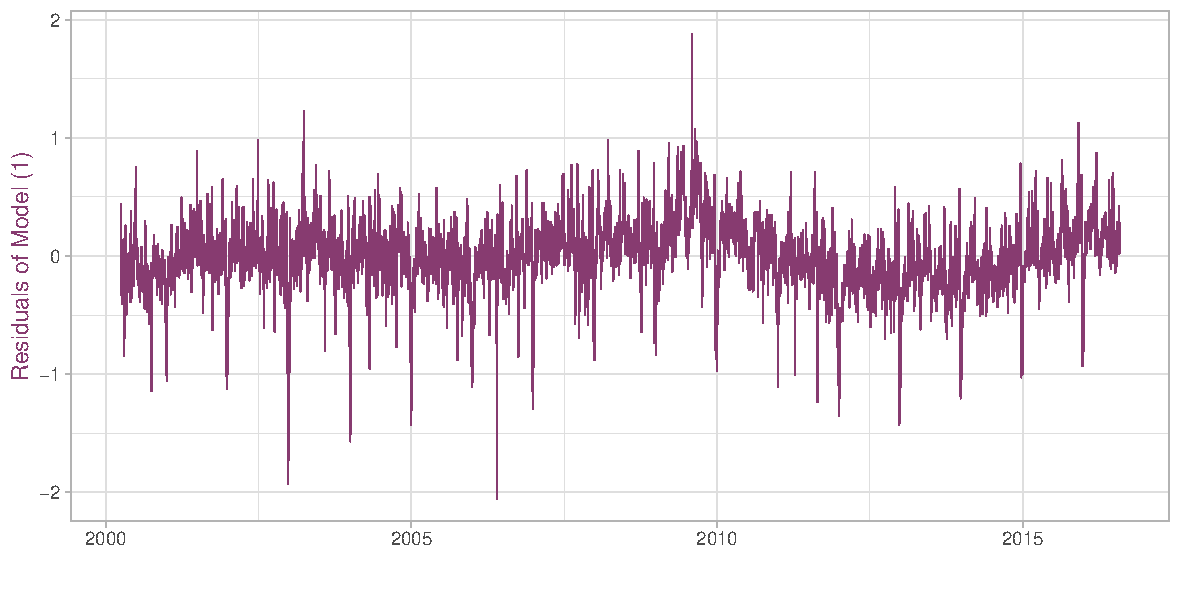
\includegraphics[width=.9\columnwidth]{atlas/chart23resid.pdf}
        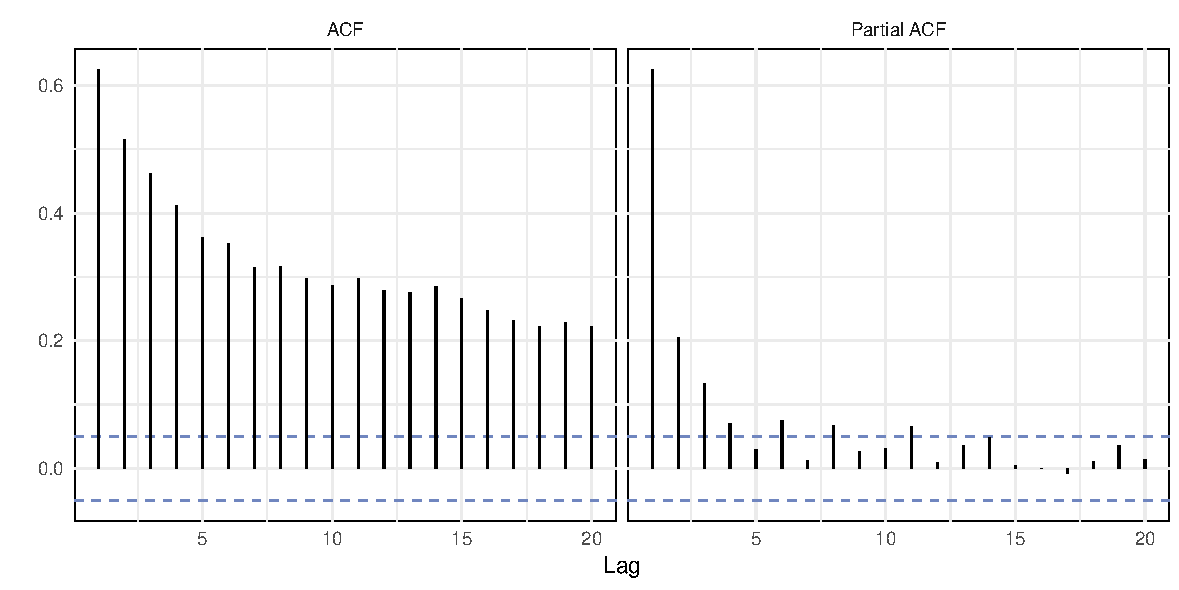
\includegraphics[width=.9\columnwidth]{atlas/chart23correl.pdf}
        \label{chart23} 
      % \wnote{The linear trend without a break is shown in \textcolor{col2}{blue}}
    \end{figure}  

\newpage
\subsection{} \label{subsec25} %%Q2.5
  



  Newey-West standard errors can be used to conduct inference in the presence of autocorrelation.\footnote{These require stationarity, which was only suggested in the evidence of section \ref{subsec25}, but will be assumed for the remaining sections.} Newey-West standard errors for model (1) are presented in Table \ref{tab2}, alongside the uncorrected standard errors. 

  \begin{table}[h!] \centering 
      \caption{Results of Model (1) with uncorrected and Newey-West standard errors} 
      \label{tab2} 
      \begin{tabular}{@{\extracolsep{5pt}}lcc} 
          \\[-1.8ex]\hline 
          \hline \\[-1.8ex] 
           & \multicolumn{2}{c}{\textit{Dependent variable:}} \\ 
          \cline{2-3} 
          \\[-1.8ex] & \multicolumn{2}{c}{$ln(vol)$} \\ 
          \\[-1.8ex] & Uncorrected standard errors & Newey-West standard errors \\ 
          \hline \\[-1.8ex] 
           t & 0.00046$^{***}$ & 0.00046$^{***}$ \\ 
            & (0.00001) & (0.00002) \\ 
            & & \\ 
           dt & -0.00075$^{***}$ & -0.00075$^{***}$ \\ 
            & (0.00001) & (0.00005) \\ 
            & & \\ 
           tue & 0.1639$^{***}$ & 0.1639$^{***}$ \\ 
            & (0.01435) & (0.00956) \\ 
            & & \\ 
           wed & 0.20808$^{***}$ & 0.20808$^{***}$ \\ 
            & (0.01434) & (0.01141) \\ 
            & & \\ 
           thu & 0.2514$^{***}$ & 0.2514$^{***}$ \\ 
            & (0.01435) & (0.01081) \\ 
            & & \\ 
           fri & 0.21555$^{***}$ & 0.21555$^{***}$ \\ 
            & (0.01442) & (0.0108) \\ 
            & & \\ 
           Constant & 12.31408$^{***}$ & 12.31408$^{***}$ \\ 
            & (0.01386) & (0.02816) \\ 
            & & \\ 
          \hline \\[-1.8ex] 
          \textit{Note:}  & \multicolumn{2}{r}{$^{*}$p$<$0.1; $^{**}$p$<$0.05; $^{***}$p$<$0.01} \\ 
    \end{tabular} 
  \end{table} 


The Newey-West standard errors of coefficients for both $t$ and $DT_{t}$ are greater than the uncorrected standard errors. This reflects the correction for autocorrelation that would otherwise inflate the significance of results. However, even after the correction $t$ and $DT_{t}$ are significant. 

\newpage
\subsection{} \label{subsec26} %Q26
The standard errors for days of the week decrease after the model is corrected for autocorrelation. Monday trading volume is \textit{even more} significantly different from all other days (\ie the results from Section \ref{subsec23} hold.) This result says that when we strip away any spurious autocorrelation, the days of the week effects were revealed to be stronger.

\subsection{} \label{subsec27} %%Q27
  The eveidence presented in Sections 2.1 to 2.6 indicate a long-term effect due on the volume of shares traded on the S\&P/ASX200 after the entrance of a competitor, Chi-X. Section \ref{subsec23} shows that the pre-Chi-X trend was 0.046\%, reversing to -0.028\% growth per trading day afterwards.



\end{document}




